%%% Template originaly created by Karol Kozioł (mail@karol-koziol.net) and modified for ShareLaTeX use

\documentclass[a4paper,11pt]{article}

\usepackage[utf8]{inputenc}
\usepackage{graphicx}
\usepackage{xcolor}

\renewcommand\familydefault{\sfdefault}

\usepackage{amsmath,amssymb,amsthm,textcomp}
\usepackage{enumerate}
\usepackage{multicol}
\usepackage{tikz}
\usepackage{hyperref}



\usepackage{geometry}
\geometry{total={210mm,297mm},
left=25mm,right=25mm,%
bindingoffset=0mm, top=20mm,bottom=20mm}


\linespread{1.3}

\newcommand{\linia}{\rule{\linewidth}{0.5pt}}

% custom theorems if needed
\newtheoremstyle{mytheor}
    {1ex}{1ex}{cmr}{0pt}{\scshape}{.}{1ex}
    {{\thmname{#1 }}{\thmnumber{#2}}{\thmnote{ (#3)}}}

\theoremstyle{mytheor}
\newtheorem{defi}{Definition}

% my own titles
\makeatletter
\renewcommand{\maketitle}{
\begin{center}
\vspace{2ex}
{\huge \textsc{\@title}}
\vspace{1ex}
\\
\linia\\
\@author \hfill \@date
\vspace{4ex}
\end{center}
}
\makeatother
%%%

% custom footers and headers
\usepackage{fancyhdr}
\pagestyle{fancy}
\lhead{}
\chead{}
\rhead{}
\lfoot{Building a Burglar Alarm with Arduino}
\cfoot{}
\rfoot{Page \thepage}
\renewcommand{\headrulewidth}{0pt}
\renewcommand{\footrulewidth}{0pt}
%

% code listing settings
\usepackage{listings}
\lstset{
    language=c,
    basicstyle=\ttfamily\small,
    aboveskip={1.0\baselineskip},
    belowskip={1.0\baselineskip},
    columns=fixed,
    extendedchars=true,
    breaklines=true,
    tabsize=4,
    prebreak=\raisebox{0ex}[0ex][0ex]{\ensuremath{\hookleftarrow}},
    frame=leftline,
    showtabs=false,
    showspaces=false,
    showstringspaces=false,
    keywordstyle=\color[rgb]{0.627,0.126,0.941},
    commentstyle=\color[rgb]{0.133,0.545,0.133},
    stringstyle=\color[rgb]{0.60,0,0},
    numbers=left,
    numberstyle=\small,
    stepnumber=1,
    numbersep=10pt,
    captionpos=t,
    escapeinside={},
    morekeywords={EEPROM, irrecv, lcd, makeTime, breakTime, time_t, TimeElements, pinMode, digitalWrite, attachInterrupt, setTime, delay, LiquidCrystal, IRrecv, decode_results},
    prebreak= \space,
    postbreak   = \space
}

\hypersetup{%
  colorlinks=true,% hyperlinks will be coloured
  linkcolor=black,% hyperlink text will be green
  linkbordercolor=red,% hyperlink border will be red
}

\usepackage{parskip}

% COLOURS %
\definecolor{inlinebackground}{RGB}{252, 252, 252}

% COMMANDS %
\newcommand{\inlinecode}[1]{\colorbox{inlinebackground}{\lstinline[basicstyle=\ttfamily\color{black}]|#1|}}

%%%----------%%%----------%%%----------%%%----------%%%

\begin{document}

\title{CS3514 C Programming for Microcontrollers Report}

\author{Colm Cahalane}

\date{28/11/2015}

\maketitle

\tableofcontents
\newpage

\section{Introduction}

The goal of this project was to construct a burglar alarm with some basic functionality using C and the Arduino framework for microcontrollers.

Some basic restrictions and requirements that were to be placed on the project were:

\begin{itemize}
\item The burglar alarm should be standalone and shouldn't need a computer to run.
\item The burglar alarm should have a settable clock with date and time.
\item The burglar alarm must support multiple zones:
\begin{itemize}
\item A digital zone, which can be active on high or low.
\item An analog zone, with a variable threshold that can be set by user.
\item An entry-exit zone that allows a user to enter a PIN number and not set off the alarm - or allow a user to arm the system and exit during a grace period.
\item A continuous monitoring zone that triggers on the high → low transition.
\end{itemize}
\item The burglar alarm must have a number of persistent settings stored in memory.
\item The burglar alarm should have a basic PIN login system.
\begin{itemize}
\item There should be a separate administrator level for making settings.
\end{itemize}
\item The burglar alarm should have the ability to store logs in EEPROM. A registered administrator should be able to view these logs on screen.
\end{itemize}

We were given a basic Arduino Duemilanove kit with which to construct the project which included an IR Remote and receiver, 2x16 character LCD Display, buttons to use as triggers, a potentiometer for analogue input, some LED lights and buzzers, a breadboard and a collection of wires.
\newpage
\section{Requirements\textbackslash Analysis\textbackslash Design}

\subsection{What are we building?}

As our group interpreted the project specifications, hardware-wise, we're looking to build a device that relays sensors for the four zones and a receiver for the IR remote to the Arduino.

The digital zones and entry-exit zones here will be activated by buttons, as that's the most simple implementation of such. Ideally, we'd like to have some sort of IR sensor for the entry-exit zone, but this is complicated by our use of IR for the remote.

The Continuous Monitoring Zone behaves like a sort of anti-tamper device; it's attached directly to a source of 5V. If the connection is broken and a high → low transition occurs on this signal, an interrupt should be triggered in software.

In return, output is to be handled by a single-pin output for a buzzer or LED and a more detailed output through the LCD display.

Ideally, for digital inputs, it would be best that we could implement these as triggering interrupts.

The goal of the project is that a user can interface with the alarm's options and settings clearly using the LCD and remote, so inputs and outputs related to operating the device should be kept very simple.

Most of the alarm's other functionality, such as timekeeping, permanent storage etc. can be implemented purely in software.

In the below table and figure we'll describe the hardware implementation and design we settled on as a group.

\begin{figure}[h]
\caption{A diagram, generated using Fritzing, that shows the hardware design we decided on.}
\centering
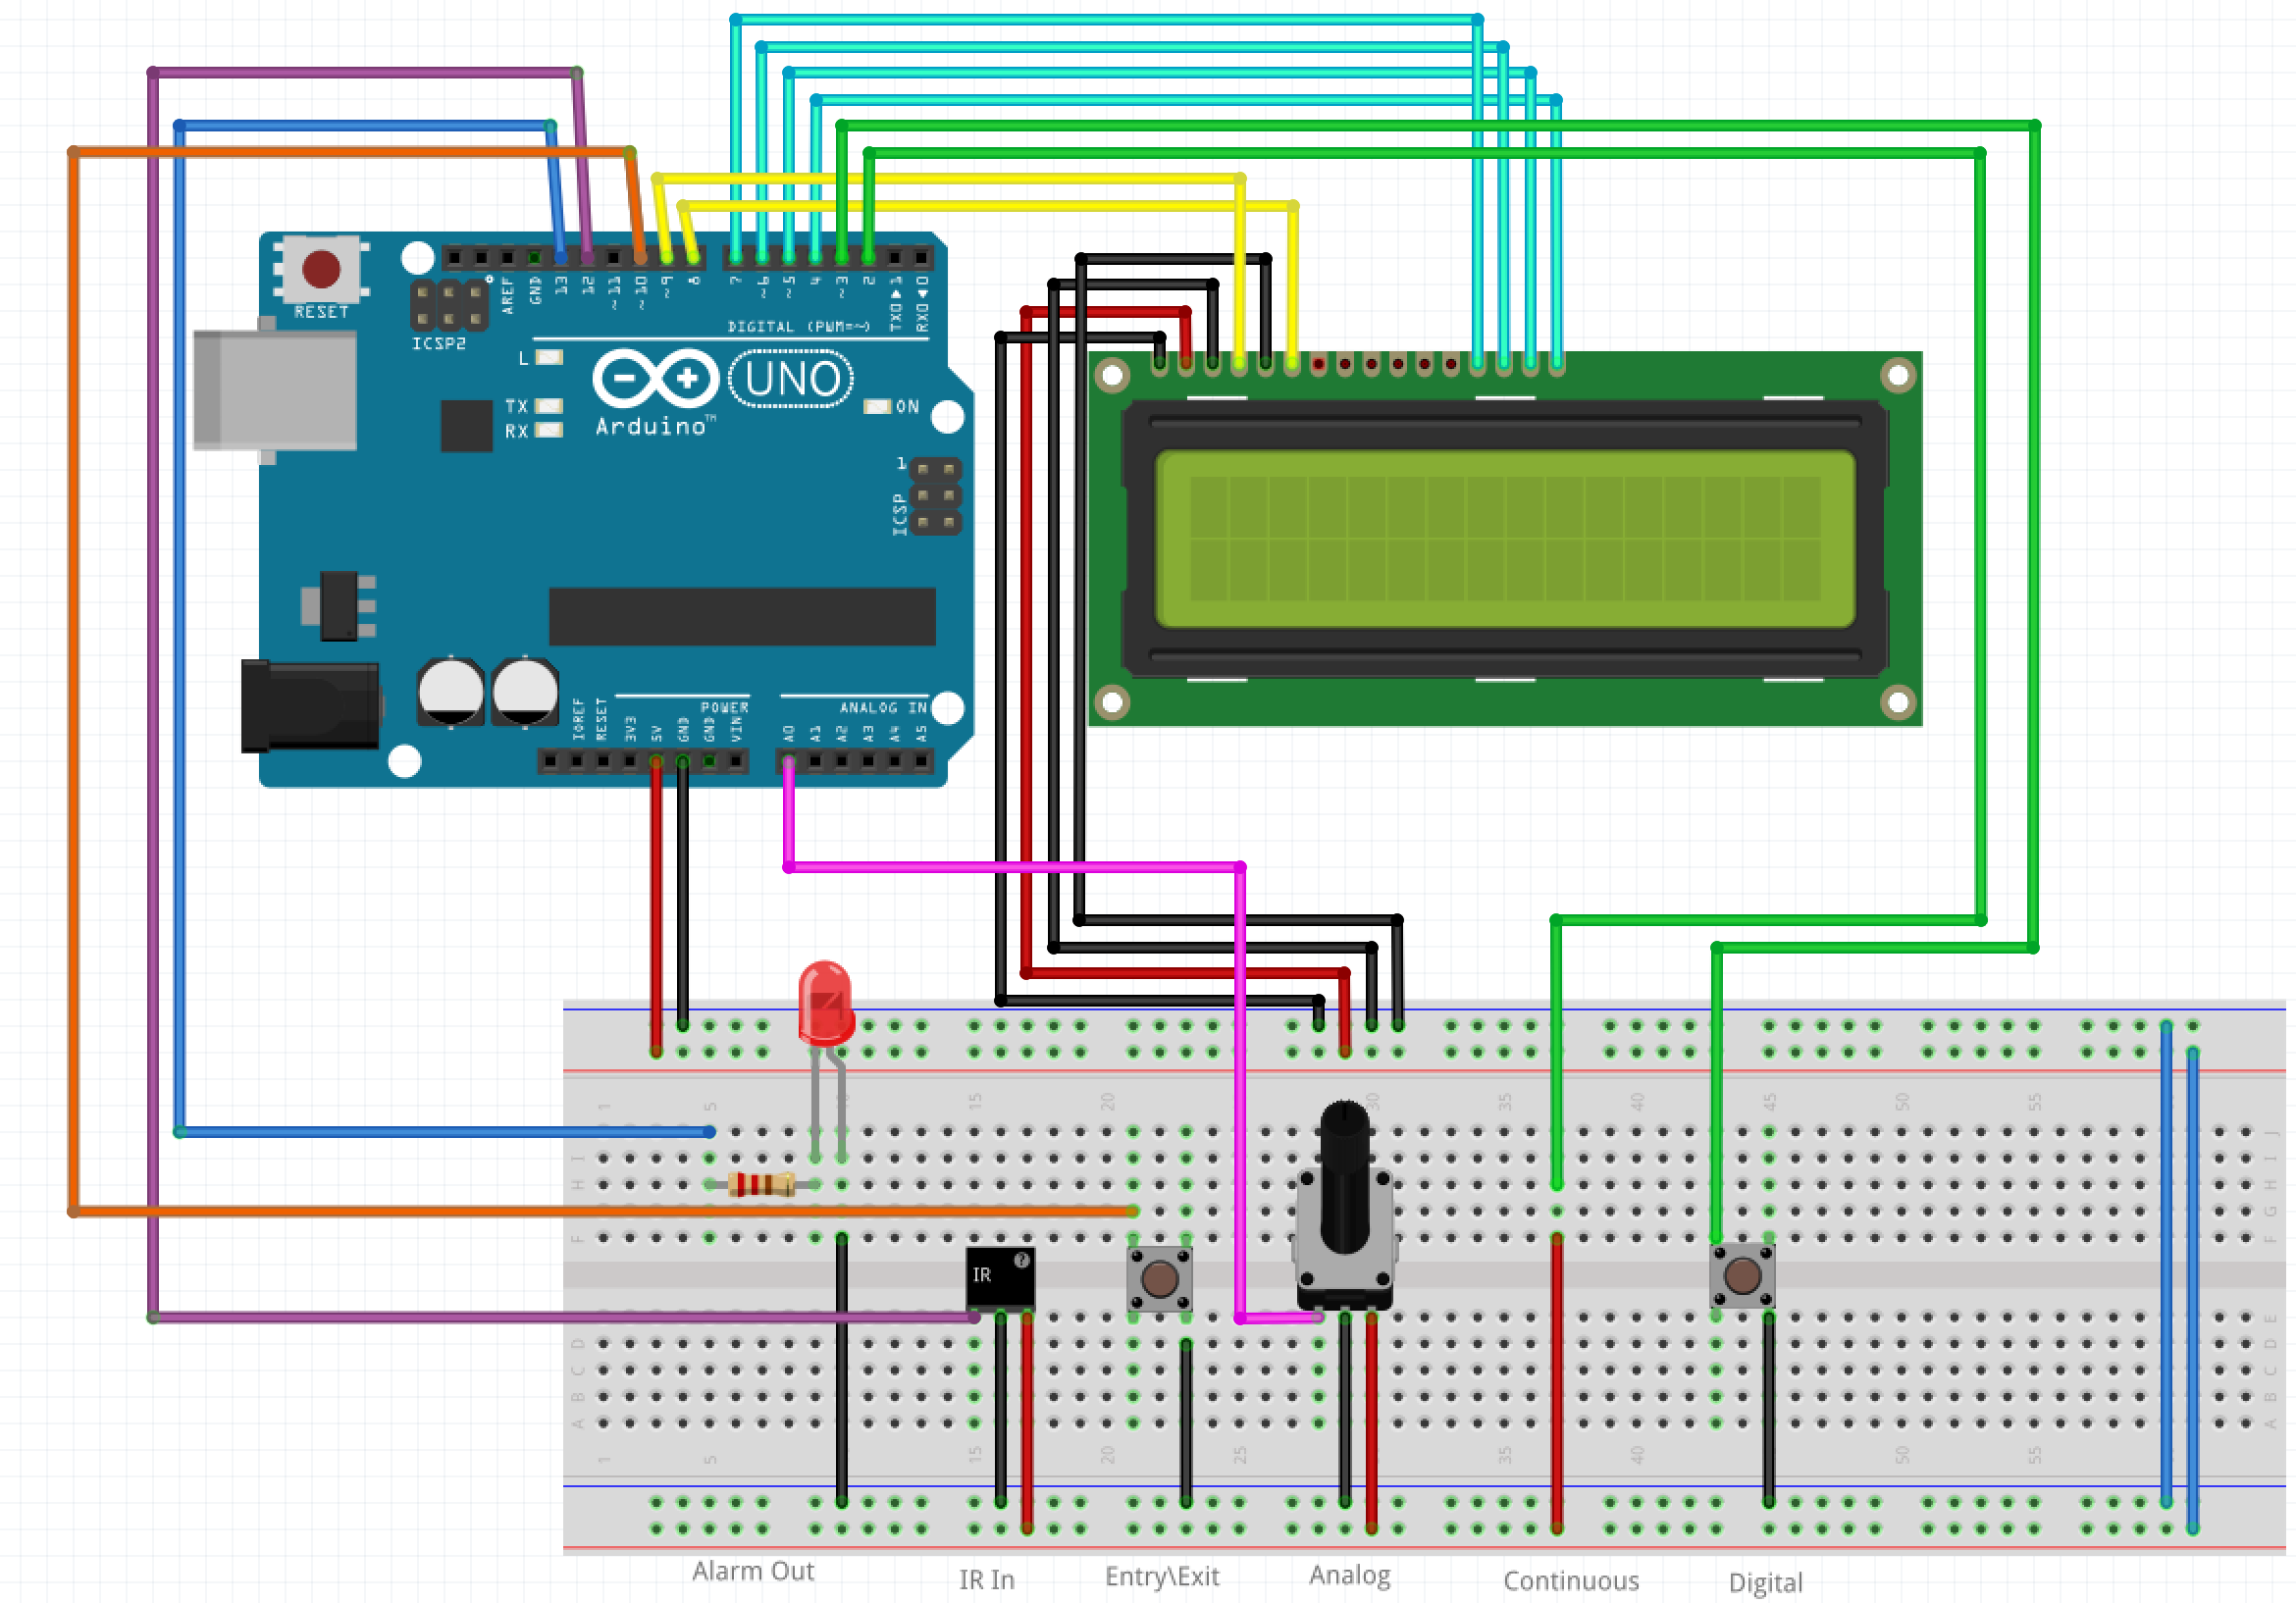
\includegraphics[width=\textwidth]{design}
\end{figure}

\begin{table}[h]
\centering
\caption{A list of the Arduino's pins in use, and how we're using them.}
\label{Pins}
\begin{tabular}{lll}
Pin \# & Mode                   & Function              \\
2      & Input (Interrupt)      & Continuous Monitoring \\
3      & Input (Interrupt)      & Digital Zone          \\
4      & Output (LiquidCrystal) & LCD                   \\
5      & Output (LiquidCrystal) & LCD                   \\
6      & Output (LiquidCrystal) & LCD                   \\
7      & Output (LiquidCrystal) & LCD                   \\
8      & Output (LiquidCrystal) & LCD                   \\
9      & Output (LiquidCrystal) & LCD                   \\
10     & Input                  & Entry/Exit Zone       \\
12     & Input (IRRemote)       & IR Sensor             \\
13     & Output                 & Alarm Output          \\
A0     & Analog Input           & Analog Zone          
\end{tabular}
\end{table}

\newpage

\subsection{What are the features we're building?}
We'll need to build software that monitors and responds to the aforementioned zones.

As indicated in the introduction, we're looking to build a number of useful features on top of the hardware that we've designed. We'll need to be able to have user login and verification, two different passwords (one for admin and one for "normal" user).

We'll need an implementation of a clock and allow the user to set the time. Timekeeping is important for our implementation of the entry/exit zone as it has certain specific hours of activity each day as well as 

We'll need a way to implement user settings and make sure that defaults are working in a way that makes sense.

The settings that we'll need to implement are:
\begin{itemize}
\item User Password
\item Admin Password
\item Threshold for Analog Zone (0 - 1024)
\item Active Hours for Entry\textbackslash Exit zone
\item Digital Zone - active high or active low
\end{itemize}

We'll need to develop a simple user privileges system and login mode to ensure that these settings are protected. Also, we shouldn't allow the alarm to be unset or disarmed until a valid login has occurred.

If any of the zone conditions are triggered, an alarm should start sounding and only be disabled if a logged-in user silences it. When an alarm sounds, we want there to be a record of this stored in permanent storage.

We'll also want these logs to be viewable by a logged-in user.

\subsection{What are the limitations we'll face?}

\subsubsection{16x2 Screen}
The 16x2 screen, allowing for 32 characters on screen at any time and of which one row is generally used for the clock, means that the user experience must suffer for functionality; we weren't able to provide for a full user menu and navigation experience. In the software design we've built commands must be learnt off or read from a manual. This is less than ideal.

\subsubsection{Timekeeping}
The Arduino doesn't have much functionality for timekeeping built in that would work in a way that suits us. While we can keep count of the number of milliseconds since the Arduino was started using {\fontfamily{cmtt}\selectfont millis()}, this doesn't work within interrupts and is not an adequate solution to implement a settable clock.

We'd have to implement a clock ourselves through a carefully written interrupt, or we could use the {\fontfamily{cmtt}\selectfont Time.h} library.

\subsubsection{Limited number of interruptable pins}
Though it would suit us to have all digital inputs handled as interrupts, the Arduino Duemilanove board only allows pins 2 and 3 to trigger interrupts. As such, we can't attach an interrupt to each of the digital, entry-exit and continuous monitoring zones. We must choose these carefully.

\subsubsection{EEPROM}
Permanent storage on an Arduino board is here provided by a library which allows for writing from and reading to EEPROM storage based on addresses. It is therefore important to us to divide the space available into EEPROM into blocks and designate specific addresses to specific functions. We must also make sure that at the same time that we have a way of checking that the values in EEPROM are set, and if not, imposing some defaults so that invalid information is not placed into the program.

\subsection{Dividing program into functional blocks.}
Based on this description of the software, we need to start to break down the program into functional blocks.

\begin{itemize}
\item A setup function that runs when the Arduino is first turned on.
\item A function which runs to check if the settings stored in EEPROM are valid and if not, set defaults.
\item Interrupt service routines for when the digital or continuous zones are breached.
\item The program's main execution loop.
\begin{itemize}
\item A section of this loop to poll the entry-exit zone and if it has been tripped, prompts the user to log in during a countdown - otherwise triggers alarm. 
\item A section of this loop to poll the analog zone and trip it if necessary
\item A function allowing a user to log in/out
\item A function allowing a logged in admin to view logs
\item A function that displays a log at an address in EEPROM
\item A function allowing a logged in admin to arm/disarm the alarm
\item A function allowing a logged in user to deactivate an active alarm.
\item A function allowing a logged in admin to set the time
\item A function allowing a logged in admin to change options stored in EEPROM
\item A function which prints the current time.
\end{itemize}
\item A set of functions available to write logs to EEPROM if an alarm is triggered.
\item A set of functions to allow settings in EEPROM to be read and changed.
\item A set of functions to interpret user input from the IR remote and return values.
\end{itemize}

\section{Implementation}

\subsection{Control-Flow Diagram}
\newpage
\begin{figure}[h!]
\caption{A general control-flow diagram layout for the program.}
\centering
\includegraphics[scale=0.345]{cfd1}
\end{figure}
\begin{figure}[h!]
\caption{A control-flow diagram the program's settings stored in EEPROM.}
\centering
\includegraphics[scale=0.3]{cfd3}
\end{figure}
\begin{figure}[h!]
\caption{A control-flow diagram for the program's time settings.}
\centering
\includegraphics[scale=0.4]{cfd2}
\end{figure}

\subsection{Coding Decisions}
\subsubsection{Timekeeping}
As outlined above in the limitations section, we had to make a decision on using a timekeeping library or write our own with interrupts. Our decision was to use {\fontfamily{cmtt}\selectfont Time.h} but the limitations of the Arduino and the small 16x2 screen meant that a user can only set the time by using the + and - buttons to increment and decrement the day/month/hour/minute etc. rather than enter the dates with numeric keys. Still, it makes up for this by giving us a universal date format that we can use in creating/storing logs, and the TimeElements structure for printing/setting time with very readable and maintainable code.

If we were to use the interrupt-based approach, this code would have been used to create a clock-based interrupt which would trigger once per second:
\begin{lstlisting}
  TCCR1A = 0;
  TCCR1B = 0;
  OCR1A = 15625;
  TCCR1B |= (1 << WGM12);
  TCCR1B |= (1 << CS10);
  TCCR1B |= (1 << CS12);
  TIMSK1 |= (1 << OCIE1A);
  sei();
\end{lstlisting}

\subsubsection{EEPROM Mapping and defaults}
We had to map out specific areas of EEPROM and the types of values that could be stored there but it took us a while to come up with a good solution for the first-boot and ensuring that the values in EEPROM were legitimate. We decided on mapping a sequence of addresses that would contain the values 'S', 'E', 'T', allowing us to have a pretty reliable indicator for if the device had been set up with the burglar alarm before. If the SET values aren't present, we'd run a function which would flash defaults.

\begin{table}[]
\centering
\caption{Locations of values stored in EEPROM and their types}
\label{EEPROM Mapping}
\begin{tabular}{lll}
Location & Information                                               & Type                        \\
0-1      & Password                                                  & unsigned int                \\
2-3      & Administrator Password                                    & unsigned int                \\
4-5      & Number Of Breaches                                        & unsigned short              \\
6-8      & 'S' 'E' 'T' values                                        & char{[}{]}                  \\
15       & lower-bound hour for entry/exit zone                      & unsigned short              \\
17       & upper-bound hour for entry/exit zone                      & unsigned short              \\
20       & Trip condition for digital zone (high/low like a boolean) & unsigned short              \\
30-32    & Threshold value for analog zone                           & unsigned int                \\
100-511  & Logging                                                   & 6 byte segments as follows: \\
L0-3     & Time of Breach                                            & unsigned long               \\
L4-5     & Zone ID                                                   & unsigned short             
\end{tabular}
\end{table}

\subsubsection{User Interaction}
As shown in the Control-Flow Diagram, the user can log in to the device, and then enter a number of settings modes from within the main loop. If the user is not logged in and attempts to enter a settings mode, they will be first asked to log in.

Handling most of this user interaction from within the main loop and not constructing an additional menu simply means that we can continue to monitor the analog and entry-exit zones actively as the user interacts with the device.

\subsubsection{Interrupts}
We use both interrupt pins to the board to ensure that active monitoring takes place at all times on certain pins. The continuous zone is set to interrupt on the high → low transition and instantly triggers the alarm. The digital zone is set to interrupt on any change and if the alarm is set, is not currently active and the digital zone switches to the condition specified by the user, the alarm is triggered.

We can not set an interrupt-based system to monitor the analog pin, and the entry-exit zone works better as a non-interrupt due to its tie-ins with the user account system and user interaction functions.


\subsection{Interesting pieces of code}

Here I'm including some particular segments of the codebase for the project that I find rather interesting or valuable in achieving elements of the project specification. Of course, the complete codebase for the project is available in the appendixes.

\subsubsection{Getting a digit value from the IR sensor}
\begin{lstlisting}
int getDigitFromIR(){
  while( 1 ){ // Loop until a button press is received
    irrecv.resume();
    while( !irrecv.decode(&results) ) { /* Wait for input! */ }
    switch(results.value)
    {
      case 0xFF6897: return 0;
      case 0xFF30CF: return 1;
      case 0xFF18E7: return 2;
      case 0xFF7A85: return 3;
      case 0xFF10EF: return 4;
      case 0xFF38C7: return 5;
      case 0xFF5AA5: return 6;
      case 0xFF42BD: return 7;
      case 0xFF4AB5: return 8;
      case 0xFF52AD: return 9;
      default:       break; // Other button press or undefined; reloop
    }
  }
}
\end{lstlisting}

\subsubsection{Checking if the EEPROM is set up right and setting defaults}
\begin{lstlisting}
int settingsSet( ){
  char first_time[3];
  EEPROM.get( FIRST_TIME_SET, first_time );
  
  // Check if the values found match our chosen string.
  return !(first_time == "SET");
}

void defaults(){
  unsigned int password = 1234, 
               admin_password = 5678, 
               analog_threshold = 100;

  unsigned short number_breaches = 0,
                 lower_bound_hour = 20,
                 upper_bound_hour = 22,
                 digital_trip_condition = 1;

  char first_time[] = "SET";
  
  // Store our default values in memory.
  EEPROM.put( FIRST_TIME_SET, first_time );
  EEPROM.put( PASSWORD, password );
  EEPROM.put( ADMIN_PASSWORD, admin_password );
  EEPROM.put( ANALOG_THRESHOLD, analog_threshold );

  EEPROM.put( NUMBER_OF_BREACHES, number_breaches );
  EEPROM.put( LOWER_TIME_BOUND, lower_bound_hour );
  EEPROM.put( UPPER_TIME_BOUND, upper_bound_hour );
  EEPROM.put( DIGITAL_CONDITION, digital_trip_condition );
}
\end{lstlisting}

\subsubsection{Printing UNIX time values}
\begin{lstlisting}
void printWithLeadingZero(int val){
  if(val < 10){
    lcd.print('0');
  }
  lcd.print(val);
}

void convertUnixToReadable( unsigned long int input_time ){
  TimeElements full_time;
  breakTime( input_time, full_time );

  printWithLeadingZero(full_time.Hour);
  lcd.print( ":" );
  printWithLeadingZero(full_time.Minute); 
  lcd.print( " " );
  printWithLeadingZero( full_time.Day );
  lcd.print("/");
  printWithLeadingZero( full_time.Month );
  lcd.print("/");
  lcd.print( full_time.Year + 1970 );
}
\end{lstlisting}

\subsubsection{User interface for modifying time}

\begin{lstlisting}
void changeTime(){
    TimeElements t;
    time_t newTime;
    breakTime(now(), t);
    
    int settingsMode = 0;
    short exitLoop = 0;

    while( !exitLoop ){
      newTime = makeTime(t);
  
      lcd.clear();
      lcd.setCursor(0,0);

      convertUnixToReadable(newTime);
    
      lcd.setCursor(0,1);
      
      if(settingsMode == HOUR){
        lcd.print("Setting HOUR");
      } else if(settingsMode == MINUTE){
        lcd.print("Setting MINUTE");
      } else if(settingsMode == DAY){
        lcd.print("Setting DAY");
      } else if(settingsMode == MONTH){
        lcd.print("Setting MONTH");
      } else if(settingsMode == YEAR){
        lcd.print("Setting YEAR");
      }

      irrecv.resume();
      while( !irrecv.decode(&results) ) { /* Wait for input! */ }
      switch(results.value){
                            // +4 should be -1, but here we avoid nevative modulo
        case 0xFF22DD: /* PREV */ settingsMode = (settingsMode+4)%5;       break;
        case 0xFF02FD: /* NEXT */ settingsMode = (settingsMode+1)%5;       break;
        case 0xFFE01F: /*  -  */
            if(settingsMode == HOUR){
              t.Hour--;
            } else if(settingsMode == MINUTE){
              t.Minute--;
            } else if(settingsMode == DAY){
              t.Day--;
            } else if(settingsMode == MONTH){
              t.Month--;
            } else if(settingsMode == YEAR){
              t.Year--;
            }
           break;
        case 0xFFA857: /*  +  */
            if(settingsMode == HOUR){
              t.Hour++;
            } else if(settingsMode == MINUTE){
              t.Minute++;
            } else if(settingsMode == DAY){
              t.Day++;
            } else if(settingsMode == MONTH){
              t.Month++;
            } else if(settingsMode == YEAR){
              t.Year++;
            }
           break;
        case 0xFFB04F: /* RET */ exitLoop = 1; lcd.clear(); break;
      }
    }

    setTime(newTime);
}
\end{lstlisting}

\subsubsection{Logging functions}
\begin{lstlisting}
/**
 * Append log to memory
 * @param time_of_breach Unix timestamp of current time
 * @param zone           Zone number that was breached
 */
void appendLog( unsigned long int time_of_breach, unsigned short zone ){

  unsigned short number_of_breaches;
  EEPROM.get( NUMBER_OF_BREACHES, number_of_breaches );

  // Increase the number of breaches
  number_of_breaches++;
  EEPROM.put( NUMBER_OF_BREACHES, number_of_breaches );

  int memory_address = LOG_MEMORY_START + (( LOG_MEMORY_START + (LOG_LENGTH * number_of_breaches) ) % 500);

  // Write our log to EEPROM
  EEPROM.put( memory_address, time_of_breach );
  memory_address += sizeof(time_of_breach);
  EEPROM.put( memory_address, (short) zone );
}

/**
 * Allows user to navigate the stored log
 * @param current_log The current log to be printed
 */
void printLog( short current_log ){
  unsigned short number_of_breaches;
  EEPROM.get( NUMBER_OF_BREACHES, number_of_breaches );

  if( current_log <= number_of_breaches && current_log != 0){
    // If we have a log to show 
    int memory_address = LOG_MEMORY_START + (( LOG_MEMORY_START + (LOG_LENGTH * current_log) ) % 500);
    
    unsigned long int time_of_breach;
    unsigned short zone;

    // Get log info
    EEPROM.get( memory_address, time_of_breach );
    memory_address += sizeof(time_of_breach);
    EEPROM.get( memory_address, zone );
    
    lcd.clear();
    switch(zone){
      case DIGITAL_ZONE:
          lcd.print( "DIGITAL ZONE");
        break;
      case ANALOG_ZONE:
          lcd.print("ANALOG ZONE");
        break;
      case CONTINUOUS_ZONE:
          lcd.print( "CONTINUOUS ZONE");
        break;
      case ENTRY_EXIT_ZONE:
          lcd.print("ENTRY/EXIT ZONE");
        break;
      default:
          lcd.print( "UNKNOWN ZONE" );
        break;
    }
    lcd.setCursor(0,1);
    convertUnixToReadable( time_of_breach );

    irrecv.resume();
    while( !irrecv.decode(&results) ) { /* Wait for input! */ }
    switch(results.value)
    {
      case 0xFF22DD: printLog( current_log - 1 );    break;
      case 0xFF02FD: printLog( current_log + 1 );    break;
      case 0xFFB04F: lcd.clear(); /* If return, just let it go */ break;
      default: printLog(current_log); // Other button press or undefined
    }
    irrecv.resume();
  } else{
    lcd.clear();
    lcd.print("NO LOGS");
    delay( 1000 );

    if( current_log > 0 )
      // If current log isn't 0, send them back a log
      printLog( current_log - 1 );
  }
}
\end{lstlisting}

\section{Evaluation}

\subsection{What went right.}

Generally speaking I consider this project to be a success. All of the most important features are implemented, the device is secure, and the code and hardware layout is generally elegant. I'm reasonably proud of how we got around some of the Arduino's specific nuances in terms of timekeeping and persistent storage in EEPROM.

Our user experience does have room for improvement (it's not immediately intuitive) but it is quite fast and responsive meaning that once a user learns their way around the system, it's fairly pleasant to do so.

Viewing logs, changing the date/time, logging in, arming the system and all of the sensors work as intended with few consequences.

We were able to demonstrate that the project implemented all of its intended functionality during the lab demonstrations.

\subsection{Room to improve.}

Given time or given the opportunity to rise above some of the issues with Arduino, some improvements could be made.

The user experience is a bit complicated. Although some of the commands correlate nicely to buttons on the remote control (ON/OFF arms or disarms the alarm, MUTE silences an ongoing alarm signal, etc.) many do not (for instance command 0 is to set the user password). We should've spent time building a menu based system for options and settings.

One notable issue is that if the analog threshold is exceeded as the system is arming, the alarm will start going off immediately after the countdown has reached zero. We should warn the user about active zones before arming the system.

One feature I wished to implement but failed to build was the ability to synchronise the clock to another device using serial communication.

It would also make sense to implement setting the clock using the number pad rather than the + / - buttons alone.

Given other hardware and further time, there would be some interesting additional functionalities we could build. Using a GSM or Ethernet shield, we could make this a connected device that would interface with other devices. It'd be interesting to implement some web server functionality and allow for the viewing of logs or the administration of the device over the network. 

\section{Appendix 1: Complete Code}
Contains previously mentioned code and comments.

\begin{lstlisting}
#include <EEPROM.h>
#include <Time.h>  
#include <IRremote.h>
#include <LiquidCrystal.h>

/**
 * @author Colm Cahalane <113326986>
 * @author Evan Smith <113300626>
 *
 * Build a burglar alarm --- The task for the project 
 * was to build a device, using an arduino, that could 
 * monitor several different types of zones, log alarm
 * trips and allow for user and admin interaction via 
 * an LCD. When an alarm condition is met, a buzzer 
 * or LED will go off indicating as such.
 * 
 * Pins
 * ====
 * 
 * Digital
 * -------
 * 
 * 2 (interrupt) : Continuous Zone 
 * 3 (interrupt) : Digital Zone
 * 4 : LCD Screen 
 * 5 : LCD Screen
 * 6 : LCD Screen
 * 7 : LCD Screen
 * 8 : LCD Screen
 * 9 : LCD Screen
 * 10: Entry/Exit Zone
 * 12: IR Sensor
 * 13: ALARM
 * 
 * Analog
 * ------
 * 0 : Analog Zone 1
 *
 * IR Remote Layout
 * ----------------
 *
 * EQ : Enter password (4-Digit Pin)
 * Return : Return to standard menu
 * Play/Pause : Navigate Log
 *   Next     : Next log
 *   Prev     : Previous log
 * Mute       : Turn off alarm
 * Power      : Set/unset the alarm
 * 0  : Set user password
 * 1  : Set admin password
 * 2  : Set lower bound hour for entry/exit zone
 * 3  : Set upper bound hour for entry/exit zone
 * 4  : Set digital activate condition
 * 5  : Set analog threshold
 *
 * EEPROM Mapping
 * --------------
 * 0 - 1 : password (unsigned int)
 * 2 - 3 : admin password (unsigned int)
 * 4 - 5 : number of breaches (unsigned short)
 * 6 - 8 : first-time settings ("set" or anything else)
 *
 *  Entry/Exit (Zone 0)
 *    15     : lower-bound hour (unsigned short)
 *    16     : upper-bound hour (unsigned short)
 *
 *  Digital (Zone 1)
 *    20    : trip condition (unsigned short)
 *    
 *  Analog  (Zone 2)
 *    30 - 32 : threshold (unsigned int)
 *
 * 100 - 511 : Logging
 *   Bit Mapping (6 bytes each):
 *   0 - 3 : time (unsigned long int)
 *   4 - 5 : zone (unsigned short)
 *   
 *   
 */

#define PASSWORD              0     // 4 digit pin
#define ADMIN_PASSWORD        2     // 4 digit pin
#define NUMBER_OF_BREACHES    4
#define FIRST_TIME_SET        6

// ~~~~~ ENTRY / EXIT ZONE ~~~~~
#define ENTRY_EXIT_ZONE       0
#define ENTRY_EXIT_PIN        10
#define LOWER_TIME_BOUND      15     // Hour (2 digits max)
#define UPPER_TIME_BOUND      16     // Hour (2 digits max)

// ~~~~~~~ DIGITAL ZONE ~~~~~~~~
#define DIGITAL_ZONE          1
#define DIGITAL_CONDITION     20    // HIGH (1) or LOW (0)
#define DIGITAL_ZONE_PIN      3

 // ~~~~~~~ ANALOG ZONE ~~~~~~~~
#define ANALOG_ZONE           2
#define ANALOG_THRESHOLD      30    // short between 0 - 255
#define ANALOG_ZONE_PIN       0


 // ~~~ CONTINUOUS MON ZONE ~~~~
#define CONTINUOUS_ZONE       3
#define CONTINUOUS_ZONE_PIN   2

 // ~~~~~ TIME SETTING MODE ~~~~
#define HOUR 0
#define MINUTE 1
#define DAY 2
#define MONTH 3
#define YEAR 4

// ~~~~~~~~~ LOGS ~~~~~~~~~~~~~~
#define LOG_MEMORY_START  100
#define LOG_LENGTH        6

// ~~~~~~~~~~ IR ~~~~~~~~~~~~~~~
#define IR_RECV_PIN   12
IRrecv irrecv(IR_RECV_PIN);
decode_results results;

#define ALARM_PIN     13

// initialize the library with the numbers of the interface pins
LiquidCrystal lcd(9, 8, 7, 6, 5, 4);

// Used to check if current user is an admin
unsigned short is_admin = 0;

// 0 is disabled ; 1 is enabled
unsigned short alarm_set = 0;

// 0 alarm is idle ; 1 alarm is ringing
volatile unsigned short alarm_active = 0;

// 0 not logged in ; 1 logged in 
unsigned short is_user_logged_in = 0;

/**
 * Prints the current time to the LCD
 */
void printTime(){
  lcd.setCursor(0, 0);
  convertUnixToReadable(now());
}

/**
 * Pads and prints an integer with 0s
 * @param val Integer to pad
 */
void printWithLeadingZero(int val){
  if(val < 10){
    lcd.print('0');
  }
  lcd.print(val);
}

/**
 * Set the time
 */
void changeTime(){
    TimeElements t;
    time_t newTime;
    breakTime(now(), t);
    
    int settingsMode = 0;
    short exitLoop = 0;

    while( !exitLoop ){
      newTime = makeTime(t);
  
      lcd.clear();
      lcd.setCursor(0,0);

      lcd.print( hour(newTime) );
      lcd.print(':');
      printWithLeadingZero( minute(newTime) );

      lcd.print(' ');

      printWithLeadingZero( day(newTime) );
      lcd.print('/');
      printWithLeadingZero( month(newTime) );
      lcd.print('/');
      lcd.print( year(newTime) );

      lcd.setCursor(0,1);
      
      if(settingsMode == HOUR){
        lcd.print("Setting HOUR");
      } else if(settingsMode == MINUTE){
        lcd.print("Setting MINUTE");
      } else if(settingsMode == DAY){
        lcd.print("Setting DAY");
      } else if(settingsMode == MONTH){
        lcd.print("Setting MONTH");
      } else if(settingsMode == YEAR){
        lcd.print("Setting YEAR");
      }

      irrecv.resume();
      while( !irrecv.decode(&results) ) { /* Wait for input! */ }
      switch(results.value){
                            // +4 should be -1, but here we avoid nevative modulo
        case 0xFF22DD: /* PREV */ settingsMode = (settingsMode+4)%5;       break;
        case 0xFF02FD: /* NEXT */ settingsMode = (settingsMode+1)%5;       break;
        case 0xFFE01F: /*  -  */
            if(settingsMode == HOUR){
              t.Hour--;
            } else if(settingsMode == MINUTE){
              t.Minute--;
            } else if(settingsMode == DAY){
              t.Day--;
            } else if(settingsMode == MONTH){
              t.Month--;
            } else if(settingsMode == YEAR){
              t.Year--;
            }
           break;
        case 0xFFA857: /*  +  */
            if(settingsMode == HOUR){
              t.Hour++;
            } else if(settingsMode == MINUTE){
              t.Minute++;
            } else if(settingsMode == DAY){
              t.Day++;
            } else if(settingsMode == MONTH){
              t.Month++;
            } else if(settingsMode == YEAR){
              t.Year++;
            }
           break;
        case 0xFFB04F: /* RET */ exitLoop = 1; lcd.clear(); break;
      }
    }

    setTime(newTime);
}

int getDigitFromIR(){
  while( 1 ){
    irrecv.resume();
    while( !irrecv.decode(&results) ) { /* Wait for input! */ }
    switch(results.value)
    {
      case 0xFF6897: return 0;
      case 0xFF30CF: return 1;
      case 0xFF18E7: return 2;
      case 0xFF7A85: return 3;
      case 0xFF10EF: return 4;
      case 0xFF38C7: return 5;
      case 0xFF5AA5: return 6;
      case 0xFF42BD: return 7;
      case 0xFF4AB5: return 8;
      case 0xFF52AD: return 9;
      default:       break; // Other button press or undefined; reloop
    }
  }
}

/**
 * Attempt to log in a user, prompting
 *   them for a user or admin password
 * @return 1 if user logged in ; 0 otherwise
 */
int loginMode() {
  lcd.clear();
  lcd.print( "Login Mode");
  if( !is_user_logged_in || !is_admin ){
    // if admin is already logged in, bypass login

    lcd.clear();
    if( is_user_logged_in && !is_admin ){
      lcd.print( "Enter admin pin");
    } else {
      lcd.print( "4 Digit Pin");
    }
    delay(50);
    
    int pin_entered = 0;
    unsigned int password, admin_password;
    EEPROM.get( PASSWORD, password );
    EEPROM.get( ADMIN_PASSWORD, admin_password );

    lcd.setCursor(0, 1);
    for(int i = 0; i < 4; i++){
      int received_value = getDigitFromIR();      
      pin_entered *= 10;
      pin_entered += received_value;
      lcd.print('*');

      // Minor delay to prevent debouncing "0"s
      delay(50);
      irrecv.resume();
    }


    lcd.setCursor(0,1);
    if( !is_user_logged_in && pin_entered == password ){
      is_user_logged_in = 1;
      lcd.print( "LOGGED IN" );
    } else if( pin_entered == admin_password ){
      is_admin = 1;
      is_user_logged_in = 1;
      lcd.print( "LOGGED IN" );
    } else{
      lcd.print( "FAILED LOGIN" );
    }
    delay(1500);
  } else{
    lcd.print("You are admin");
  }
  lcd.clear();
  
  return is_user_logged_in;
}

/**
 * Append log to memory
 * @param time_of_breach Unix timestamp of current time
 * @param zone           Zone number that was breached
 */
void appendLog( unsigned long int time_of_breach, unsigned short zone ){

  unsigned short number_of_breaches;
  EEPROM.get( NUMBER_OF_BREACHES, number_of_breaches );

  // Increase the number of breaches
  number_of_breaches++;
  EEPROM.put( NUMBER_OF_BREACHES, number_of_breaches );

  int memory_address = LOG_MEMORY_START + (( LOG_MEMORY_START + (LOG_LENGTH * number_of_breaches) ) % 500);

  // Write our log to EEPROM
  EEPROM.put( memory_address, time_of_breach );
  memory_address += sizeof(time_of_breach);
  EEPROM.put( memory_address, (short) zone );
}

/**
 * Allows user to navigate the stored log
 * @param current_log The current log to be printed
 */
void printLog( short current_log ){
  unsigned short number_of_breaches;
  EEPROM.get( NUMBER_OF_BREACHES, number_of_breaches );

  if( current_log <= number_of_breaches && current_log != 0){
    // If we have a log to show 
    int memory_address = LOG_MEMORY_START + (( LOG_MEMORY_START + (LOG_LENGTH * current_log) ) % 500);
    
    unsigned long int time_of_breach;
    unsigned short zone;

    // Get log info
    EEPROM.get( memory_address, time_of_breach );
    memory_address += sizeof(time_of_breach);
    EEPROM.get( memory_address, zone );
    
    lcd.clear();
    switch(zone){
      case DIGITAL_ZONE:
          lcd.print( "DIGITAL ZONE");
        break;
      case ANALOG_ZONE:
          lcd.print("ANALOG ZONE");
        break;
      case CONTINUOUS_ZONE:
          lcd.print( "CONTINUOUS ZONE");
        break;
      case ENTRY_EXIT_ZONE:
          lcd.print("ENTRY/EXIT ZONE");
        break;
      default:
          lcd.print( "UNKNOWN ZONE" );
        break;
    }
    lcd.setCursor(0,1);
    convertUnixToReadable( time_of_breach );

    irrecv.resume();
    while( !irrecv.decode(&results) ) { /* Wait for input! */ }
    switch(results.value)
    {
      case 0xFF22DD: printLog( current_log - 1 );    break;
      case 0xFF02FD: printLog( current_log + 1 );    break;
      case 0xFFB04F: lcd.clear(); /* If return, just let it go */ break;
      default: printLog(current_log); // Other button press or undefined
    }
    irrecv.resume();
  } else{
    lcd.clear();
    lcd.print("NO LOGS");
    delay( 1000 );

    if( current_log > 0 )
      // If current log isn't 0, send them back a log
      printLog( current_log - 1 );
  }
}

/**
 * Prints out unix time in a human-readable format
 * @param  input_time Unix time input
 */
void convertUnixToReadable( unsigned long int input_time ){
  TimeElements full_time;
  breakTime( input_time, full_time );

  printWithLeadingZero(full_time.Hour);
  lcd.print( ":" );
  printWithLeadingZero(full_time.Minute); 
  lcd.print( " " );
  printWithLeadingZero( full_time.Day );
  lcd.print("/");
  printWithLeadingZero( full_time.Month );
  lcd.print("/");
  lcd.print( full_time.Year + 1970 );
}

/**
 * Exit admin mode
 */
void exitAdmin( ){
  is_admin = 0;
  logout( );
}

/**
 * Remove logged in status
 */
void logout( ){
  is_user_logged_in = 0;
  lcd.clear();
  lcd.print("Logged out");
  delay(700);
}

/**
 * Change whether the alarm can be active or not
 */
void toggleAlarmSet( ){
  if( !alarm_active ){
    lcd.clear();
    // We set the alarm at the end of the function to
    // avoid interrupts triggering the alarm
    unsigned short temp_alarm = !alarm_set;
    
    if( temp_alarm ){
      logout( );
      for (int i = 9; i < 10 && i >= 0; i--){
        lcd.clear();
        lcd.print(i);
        delay(1000);
      }
      lcd.clear();
      lcd.print( "ALARM SET" );
      delay(800);
    } else{
      lcd.print( "ALARM UNSET" );
      delay(800);
    }

    alarm_set = temp_alarm;
  }
}

/**
 * Change whether alarm is ringing or not
 */
void toggleAlarm( ){
  alarm_active = !alarm_active;

  lcd.clear();
  lcd.setCursor(0,1);
  if( alarm_set ){
    if( alarm_active ){
      lcd.print( "ALARM ACTIVE     " );
      digitalWrite( ALARM_PIN, HIGH );
    } else {
      lcd.print( "ALARM DEACTIVATED" );
      digitalWrite( ALARM_PIN, LOW );
      delay(1500);
      lcd.clear();
    }
  }
}


/**
 * Trip the digital zone if conditions are met
 */
void digitalZoneTrip( ){
  volatile unsigned short trip_condition;
  EEPROM.get( DIGITAL_CONDITION, trip_condition );

  if( trip_condition ){
    if( digitalRead( DIGITAL_ZONE_PIN ) == HIGH && !alarm_active && alarm_set ){
      toggleAlarm( );
      appendLog( now(), DIGITAL_ZONE );
    }
  } else {
    if( digitalRead( DIGITAL_ZONE_PIN ) == LOW && !alarm_active && alarm_set ){
      toggleAlarm( );
      appendLog( now(), DIGITAL_ZONE );
    }
  }
}

/**
 * Trip the continuous zone
 */
void contZoneTrip( ){
  toggleAlarm( );
  appendLog( now(), CONTINUOUS_ZONE );
}

/**
 * Trip the analog zone if higher than threshold
 */
void analogZoneTrip( ){
  unsigned int threshold;
  EEPROM.get( ANALOG_THRESHOLD, threshold );

  if( analogRead( ANALOG_ZONE_PIN ) > threshold && !alarm_active && alarm_set ){
    toggleAlarm( );
    appendLog( now(), ANALOG_ZONE );
    delay(200);
  }
}

/**
 * Allows users to set permanent option 
 *   values (stored in EEPROM)
 * @param option Option number from IR Remote
 */
void setOption( short option ){
  unsigned int address;
  unsigned short digits;
  switch( option ){
    case 0:
        lcd.print("PASSWORD");
        address = PASSWORD;
        digits = 4;
      break;
    case 1:
        lcd.print("ADMIN_PASSWORD");
        address = ADMIN_PASSWORD;
        digits = 4;
      break;
    case 2:
        lcd.print("LOWER TIME (Hour)");
        address = LOWER_TIME_BOUND;
        digits = 2;
      break;
    case 3:
        lcd.print("UPPER TIME (Hour)");
        address = UPPER_TIME_BOUND;
        digits = 2;
      break;
    case 4:
        lcd.print("DIGITAL COND 0/1");
        address = DIGITAL_CONDITION;
        digits = 1;
      break;
    case 5:
        lcd.print("ANALOG THRESH 1-255");
        address = ANALOG_THRESHOLD;
        digits = 3;
      break;
    default:
        return;
      break;
  }

  if( digits > 2 ){
    // If there are more than 2 digits, we'll need an int
    unsigned int final_value = 0;
    lcd.setCursor(0,1);
    for(int i = 0; i < digits; i++){
      int received_value = getDigitFromIR();
        final_value *= 10;
        final_value += received_value;
        lcd.print(received_value);
        // Minor delay to prevent debouncing "0"s
        delay(50);
        irrecv.resume();
    }
    EEPROM.put( address, final_value );
  } else {
    // If there are less than 2 digits, we can use a short
    unsigned short final_value = 0;
    lcd.setCursor(0,1);
    for(int i = 0; i < digits; i++){
      int received_value = getDigitFromIR();
        final_value *= 10;
        final_value += received_value;
        lcd.print(received_value);
        // Minor delay to prevent debouncing "0"s
        delay(50);
        irrecv.resume();
    }
    EEPROM.put( address, final_value );
  }
}

/**
 * Places default values in memory if it's the 
 * first time
 */
void defaults(){
  unsigned int password = 1234, 
               admin_password = 5678, 
               analog_threshold = 100;

  unsigned short number_breaches = 0,
                 lower_bound_hour = 20,
                 upper_bound_hour = 22,
                 digital_trip_condition = 1;

  char first_time[] = "SET";
  EEPROM.put( FIRST_TIME_SET, first_time );
  EEPROM.put( PASSWORD, password );
  EEPROM.put( ADMIN_PASSWORD, admin_password );
  EEPROM.put( ANALOG_THRESHOLD, analog_threshold );

  EEPROM.put( NUMBER_OF_BREACHES, number_breaches );
  EEPROM.put( LOWER_TIME_BOUND, lower_bound_hour );
  EEPROM.put( UPPER_TIME_BOUND, upper_bound_hour );
  EEPROM.put( DIGITAL_CONDITION, digital_trip_condition );
}

/**
 * Check if settings exist
 * @return 0 if not first time; 1 if first time
 */
int settingsSet( ){
  char first_time[3];

  EEPROM.get( FIRST_TIME_SET, first_time );

  return !(first_time == "SET");
}

void setup() {
  pinMode(ALARM_PIN, OUTPUT);
  pinMode(CONTINUOUS_ZONE_PIN, INPUT);
  pinMode(DIGITAL_ZONE_PIN, INPUT);
  pinMode(ENTRY_EXIT_PIN, INPUT);

  digitalWrite( ALARM_PIN, LOW );
  digitalWrite( CONTINUOUS_ZONE_PIN, LOW );
  digitalWrite( DIGITAL_ZONE_PIN, LOW );

  attachInterrupt( digitalPinToInterrupt(DIGITAL_ZONE_PIN), digitalZoneTrip, CHANGE  );
  attachInterrupt( digitalPinToInterrupt(CONTINUOUS_ZONE_PIN), contZoneTrip, FALLING );

  int first_time = settingsSet( );

  if( first_time ){
    defaults();
  }

  alarm_set = 0;
  
  setTime( 1447854337 );
      
  irrecv.enableIRIn(); 

  lcd.begin(16, 2);
}

void loop() {

  /**
   * Trip the Entry/Exit zone as necessary
   */
  if( digitalRead(ENTRY_EXIT_PIN) == HIGH ){
    unsigned short lower, upper, currentHour;
    EEPROM.get( LOWER_TIME_BOUND, lower );
    EEPROM.get( UPPER_TIME_BOUND, upper );
    currentHour = hour();

    lcd.clear();
    lcd.print("Plz login (EQ)");
    long start_time = millis();
    lcd.setCursor(0,1);
    while( (millis() - start_time) < 20000 ){
       
      irrecv.resume();
      delay(300);
      if(irrecv.decode(&results)){  
        if( results.value == 0xFF906F ){
          if( !is_user_logged_in ){
           loginMode( );
          }
          lcd.clear();
          lcd.print("Crisis averted");
          delay(800);
          break;
        }
      }
      lcd.clear();
      lcd.print("Plz login (EQ)");
      lcd.setCursor(0,1);
      lcd.print( 20 - ((millis() - start_time) / 1000) );
    }
    irrecv.resume(); 

    if( !alarm_active && alarm_set && !( currentHour <= lower && currentHour >= upper) ){
      // If current hour is not between the upper and lower bound
      // then activate the alarm
      toggleAlarm( );
      appendLog( now(), ENTRY_EXIT_ZONE );
      delay( 200 );
    }
  }
  
  analogZoneTrip( );

  if( irrecv.decode(&results) ) {
    switch(results.value)
    {
      case 0xFF906F: 
          // EQ
          loginMode();
        break;
      case 0xFFA25D:
          // POW
          if( !alarm_active && ( is_user_logged_in || loginMode() ) )
            toggleAlarmSet( );
        break;
      case 0xFFE21D:
          // MUTE
          if( alarm_active && ( is_user_logged_in || loginMode() ) ){
            toggleAlarm();
          }
        break;
      case 0xFFC23D: 
          /* PLAY/PAUSE */ 
          if( is_user_logged_in || loginMode() )
            printLog( 1 ); 
        break;
      case 0xFF9867:
          /* 100+ */
          if(is_user_logged_in || loginMode() ){
            changeTime();
          }
        break;

      case 0xFFB04F:
          // RET
          if( is_admin ){
            exitAdmin( );
          } else if( is_user_logged_in ){
            logout();
          }
        break;

      /* SET OPTION VALUES */
      case 0xFF6897: 
          if( is_admin || ( loginMode( ) && is_admin ) )
            setOption( 0 );
        break;
      case 0xFF30CF: 
          if( is_admin || ( loginMode( ) && is_admin ) )
            setOption( 1 );
        break;
      case 0xFF18E7: 
          if( is_admin || ( loginMode( ) && is_admin ) )
            setOption( 2 );
        break;
      case 0xFFFFFF: 
          if( is_admin || ( loginMode( ) && is_admin ) )
            setOption( 3 );
        break;
      case 0xFF10EF: 
          if( is_admin || ( loginMode( ) && is_admin ) )
            setOption( 4 );
        break;
      case 0xFF38C7: 
          if( is_admin || ( loginMode( ) && is_admin ) )
            setOption( 5 );
        break;

      default: 
    }

    irrecv.resume(); // Receive the next value
  } else {
      printTime();
  }

}
\end{lstlisting}

\section{Appendix 2: User Manual}
The RainbowTables Burglar Alarm is an arduino-based alarm system. As such, it will need to be powered by some external power source or by USB, but it will not need to be connected to a computer to function. As soon as it is powered on, it will set some default settings.

It by default monitors four zones, an entry-exit zone, a digital zone, an analog zone, and an anti-tampering device located within the alarm.

To log into the system, you can press the EQ button, and enter one of the default passwords; for basic user it's {\fontfamily{cmtt}\selectfont 1234} and for administrator it's {\fontfamily{cmtt}\selectfont 5678}.

Once you're logged in as administrator, you can change these passwords. For user password, press 0 to change. For administrator, press 1.

There are some other settings you can change from this screen. Pressing 2 allows you to set the lower bound hour for the entry-exit zone, and pressing 3 allows you to set the upper bound hour. What this means is that you can set the time during which the entry-exit zone is monitoring actively and can trigger an alarm. These bounds are set by giving a number from 0 to 24 indicating the hours at which it is active. By default, it is active from 20:00 to 22:00.

You can also set if the digital zone should be triggered on a switch to low or high. This can be changed by pressing 4. By default, it activates on High. If you wish for it to activate on Low, set this value to 0. Set this value back to 1 if you would like to restore the default behaviour.

You can also set the sensitivity of the analog zone - a number from 0 to 1024 indicating the value at which the analog zone is triggered. 0 represents no voltage being carried, and 1024 represents a 5 volt charge. You can set this value by pressing 5. By default, this value is set to 100.

To set the clock on the device, press the 100+ button. Navigate between the Day/Month/Year\-/Hour/Minute settings using the Previous and Next buttons and use the + and - buttons to adjust these values. Press the return button to save settings.

To arm the alarm system, press the power button. Note that you will be logged out and given a countdown for which to exit the area as monitoring will begin after this period.

If you trigger an alarm, you can press the mute button to silence it. You will be asked to log in if you are not already. If you trigger the Entry-Exit zone, you have a twenty second window to log in with a valid password (by pressing EQ) before the alarm becomes triggered.

When an alarm is triggered, a log is recorded of the incident. To view the logs, press the Play-Pause button. Using the Previous and Next buttons, you can navigate through a log of breaches.

To log out, simply press the return button.

If the device is powered off or plugged out, the clock will be reset but the settings and logs will remain. 

\section{Appendix 3: Project Plan}
\begin{enumerate}
    \item Review description and decide on possible hardware design
    \item Create a basic hardware design (with Fritzing) which implements each sensor zone.
    \item Ensure that the pin layout chosen fits some requirements (interrupts limitation etc.)
    \item Construct this hardware.
    \item Design a basic implementation of software that monitors and reacts to the sensor zones.
    \item Test this implementation of hardware and software.
    \item Implement and test an LCD clock on top of the alarm system.
    \item Implement and test a basic user interaction system using the IR remote on top of the above.
    \item Implement and test a user account and privileges system, allowing users to activate/deactivate the alarm, set the clock, etc.
    \item Map out locations within EEPROM where values will be stored.
    \item Implement and test integrity checking and defaults.
    \item Allow users to change these settings and store their values in EEPROM. Test this.
    \item Implement logging functionality and test.
    \item Run a complete test of all functionality.
    \item Make necessary changes to respond to any limitations or issues that arose in testing.
    \item Finalize code and design, test, and present in class.
\end{enumerate}

\end{document}